\documentclass[10pt,landscape]{article}
\usepackage[usenames,dvips,pdftex]{color}
\usepackage{multicol}
\usepackage{calc}
\usepackage{ifthen}
\usepackage[pdftex]{color,graphicx}
\usepackage[landscape]{geometry}
\usepackage{hyperref}
\hypersetup{colorlinks=true, filecolor=black, linkcolor=black, urlcolor=blue, citecolor=black}
\graphicspath{{./images/}}


% To make this come out properly in landscape mode, do one of the following
% 1.
%  pdflatex latexsheet.tex
%
% 2.
%  latex latexsheet.tex
%  dvips -P pdf  -t landscape latexsheet.dvi
%  ps2pdf latexsheet.ps


% If you're reading this, be prepared for confusion.  Making this was
% a learning experience for me, and it shows.  Much of the placement
% was hacked in; if you make it better, let me know...


% 2008-04
% Changed page margin code to use the geometry package. Also added code for
% conditional page margins, depending on paper size. Thanks to Uwe Ziegenhagen
% for the suggestions.

% 2006-08
% Made changes based on suggestions from Gene Cooperman. <gene at ccs.neu.edu>


% To Do:
% \listoffigures \listoftables
% \setcounter{secnumdepth}{0}


% This sets page margins to .5 inch if using letter paper, and to 1cm
% if using A4 paper. (This probably isn't strictly necessary.)
% If using another size paper, use default 1cm margins.
\ifthenelse{\lengthtest { \paperwidth = 11in}}
	{ \geometry{top=.40in,left=.5in,right=.5in,bottom=.40in} }
	{\ifthenelse{ \lengthtest{ \paperwidth = 297mm}}
		{\geometry{top=1cm,left=1cm,right=1cm,bottom=1cm} }
		{\geometry{top=1cm,left=1cm,right=1cm,bottom=1cm} }
	}

% Turn off header and footer
\pagestyle{empty}


% Redefine section commands to use less space
\makeatletter
\renewcommand{\section}{\@startsection{section}{1}{0mm}%
                                {-0mm} %plus -.5mm minus -.5mm}%
                                {0.5mm}%x
                                {\normalfont\large\bfseries}}
\renewcommand{\subsection}{\@startsection{subsection}{2}{0mm}%
                                {-0mm}%
                                {0.5ex plus .2ex}%
                                {\normalfont\normalsize\bfseries}}
\renewcommand{\subsubsection}{\@startsection{subsubsection}{3}{0mm}%
                                {-1mm}%
                                {1ex plus .2ex}%
                                {\normalfont\small\bfseries}}
\makeatother

% Define BibTeX command
\def\BibTeX{{\rm B\kern-.05em{\sc i\kern-.025em b}\kern-.08em
    T\kern-.1667em\lower.7ex\hbox{E}\kern-.125emX}}

% Don't print section numbers
\setcounter{secnumdepth}{0}


\setlength{\parindent}{0pt}
\setlength{\parskip}{0pt plus 0.5ex}


% -----------------------------------------------------------------------

\begin{document}

\raggedright
\footnotesize
\begin{multicols}{3}


% multicol parameters
% These lengths are set only within the two main columns
%\setlength{\columnseprule}{0.25pt}
\setlength{\premulticols}{1pt}
\setlength{\postmulticols}{1pt}
\setlength{\multicolsep}{1pt}
\setlength{\columnsep}{2pt}

\begin{center}
     \Large{\textbf{ROS Cheat Sheet}} \\
\end{center}
\newlength{\MyLen}
\settowidth{\MyLen}{\texttt{letterpaper}/\texttt{a4paper} \ }

%\section{Filesystem Concepts}
%\begin{tabular}{@{}p{\the\MyLen}%
 %               @{}p{\linewidth-\the\MyLen}@{}}
%\texttt{\href{http://www.ros.org/wiki/Packages}{package}}   & The lowest level of ROS software organization. \\
%\texttt{\href{http://www.ros.org/wiki/Manifest}{manifest}}  & Description of a ROS package. \\
%\texttt{\href{http://www.ros.org/wiki/Stack}{stack}} & Collections of ROS packages that form a higher-level library. \\
%\texttt{\href{http://www.ros.org/wiki/Stack Manifest}{stack manifest}}  & Description of a ROS stack.
%\end{tabular}

\section{Filesystem Command-line Tools}
\vspace{1.5mm}
\begin{tabular}{@{}p{\the\MyLen}%
                @{}p{\linewidth-\the\MyLen}@{}}
\texttt{\href{http://www.ros.org/wiki/rospack}{rospack}}/\texttt{rosstack} & A tool inspecting \href{http://www.ros.org/wiki/Packages}{packages}/\href{http://www.ros.org/wiki/Stack}{stacks}. \\
\texttt{roscd} & Changes directories to a package or stack. \\
\texttt{rosls} & Lists package or stack information. \\
\texttt{\href{http://www.ros.org/wiki/catkin}{catkin\_create\_pkg}} & Creates a new ROS package. \\
\texttt{\href{http://www.ros.org/wiki/catkin}{catkin\_make}} & Builds a ROS Catkin package (Run at the root of your workspace).\\
\texttt{\href{http://www.ros.org/wiki/rosdep}{rosdep}} & Installs ROS package system dependencies.\\
\texttt{\href{http://www.ros.org/wiki/roscreate}{roscreate}-stack} & Creates a new ROS stack.\\
\texttt{\href{http://www.ros.org/wiki/roscreate}{roscreate}-pkg} & Creates a new ROS package. \\
\texttt{\href{http://www.ros.org/wiki/rosmake}{rosmake}} & Builds a ROS package.\\
\texttt{\href{http://www.ros.org/wiki/roswtf}{roswtf}} & Displays a errors and warnings about a running ROS system or launch file.\\
\texttt{\href{http://www.ros.org/wiki/rxdeps}{rxdeps}} & Displays package structure and dependencies.\\
\end{tabular}

\begin{tabbing}
Us\=age:\\
\> \texttt{\$ rospack find [package]}\\
\> \texttt{\$ roscd [package[/subdir]]}\\
\> \texttt{\$ rosls [package[/subdir]]}\\
\> \texttt{\$ catkin\_create\_pkg [package\_name]}\\
\> \texttt{\$ catkin\_make}\\
\> \texttt{\$ rosdep install [package]}\\
\> \texttt{\$ roswtf or roswtf [file]}\\
\> \texttt{\$ rxdeps [options]}
\end{tabbing}

\vspace{-1mm}
\section{Common Command-line Tools}
\subsection{\href{http://www.ros.org/wiki/roscore}{roscore}}
A collection of \href{http://www.ros.org/wiki/Nodes}{nodes} and programs that are pre-requisites of a ROS-based system. You must have a roscore running in order for ROS nodes to communicate.\\
\vspace{-1.5mm}
\begin{tabbing}
ro\=score is currently defined as:\\
\> \texttt{\href{http://www.ros.org/wiki/Master}{master}}\\
\> \texttt{\href{http://www.ros.org/wiki/Parameter Server}{parameter server}}\\
\> \texttt{\href{http://www.ros.org/wiki/rosout}{rosout}}
\end{tabbing}
\begin{tabbing}
Us\=age:\\
\> \texttt{\$ roscore}
\end{tabbing}

\vspace{-1.5 mm}
\subsection{\href{http://www.ros.org/wiki/rosmsg}{rosmsg/rossrv}}
rosmsg/rossrv displays Message/Service (msg/srv) data structure definitions.\\
Commands: \\
\begin{tabular}{@{}p{\the\MyLen}%
                @{}p{\linewidth-\the\MyLen}@{}}
\texttt{rosmsg show}    & Display the fields in the msg. \\
\texttt{rosmsg users}    & Search for code using the msg. \\
\texttt{rosmsg md5}    & Display the msg md5 sum. \\
\texttt{rosmsg package} & List all the messages in a package. \\
\texttt{rosnode packages}    & List all the packages with messages.
\end{tabular}
\begin{tabbing}
E\=x\=amples:\\
\> Display the Pose msg:\\
\> \> \texttt{\$ rosmsg show Pose}\\
\> List the messages in nav\_msgs:\\
\> \> \texttt{\$ rosmsg package nav\_msgs}\\
\> List the files using sensor\_msgs/CameraInfo:\\
\> \> \texttt{\$ rosmsg users sensor\_msgs/CameraInfo}
\end{tabbing}



\vspace{-1.5 mm}
\subsection{\href{http://www.ros.org/wiki/rosrun}{rosrun}}
rosrun allows you to run an executable in an arbitrary package without having to cd (or roscd) there first.\\
\begin{tabbing}
Us\=age:\\
\> \texttt{\$ rosrun package executable}
\end{tabbing}
\vspace{-3.5mm}
\begin{tabbing}
E\=x\=ample:\\
\> Run turtlesim:\\
\> \> \texttt{\$ rosrun turtlesim turtlesim\_node}\\
\end{tabbing}

\vspace{-1.5 mm}
\subsection{\href{http://www.ros.org/wiki/rosnode}{rosnode}}
Displays debugging information about ROS nodes, including publications, subscriptions and connections.\\
\vspace{2.5 mm}
Commands: \\
\begin{tabular}{@{}p{\the\MyLen}%
                @{}p{\linewidth-\the\MyLen}@{}}
\texttt{rosnode ping}    & Test connectivity to node. \\
\texttt{rosnode list}    & List active nodes. \\
\texttt{rosnode info}    & Print information about a node. \\
\texttt{rosnode machine} & List nodes running on a particular machine. \\
\texttt{rosnode kill}    & Kills a running node.
\end{tabular}
\begin{tabbing}
E\=x\=amples:\\
\> Kill all nodes:\\
\> \> \texttt{\$ rosnode kill -a}\\
\> List nodes on a machine:\\
\> \> \texttt{\$ rosnode machine aqy.local}\\
\> Ping all nodes:\\
\> \> \texttt{\$ rosnode ping --all}
\end{tabbing}


\vspace{-1.5 mm}
\subsection{\href{http://www.ros.org/wiki/roslaunch}{roslaunch}}
Starts ROS nodes locally and remotely via SSH, as well as setting parameters on the parameter server.\\
\begin{tabbing}
E\=x\=amples:\\
\> Launch on a different port:\\
\> \> \texttt{\$ roslaunch -p 1234 package filename.launch}\\
\> Launch a file in a package:\\
\> \> \texttt{\$ roslaunch package filename.launch}\\
\> Launch on the local nodes:\\
\> \> \texttt{\$ roslaunch --local package filename.launch}
\end{tabbing}


\vspace{-1.5 mm}
\subsection{\href{http://www.ros.org/wiki/rostopic}{rostopic}}
A tool for displaying debug information about ROS \href{http://www.ros.org/wiki/Topics}{topics}, including publishers, subscribers, publishing rate, and messages.\\
\vspace{2.5 mm}
Commands: \\
\begin{tabular}{@{}p{\the\MyLen}%
                @{}p{\linewidth-\the\MyLen}@{}}
\texttt{rostopic bw}   & Display bandwidth used by topic. \\
\texttt{rostopic echo}   & Print messages to screen. \\
\texttt{rostopic hz}   & Display publishing rate of topic. \\
\texttt{rostopic list}   & Print information about active topics. \\
\texttt{rostopic pub}   & Publish data to topic. \\
\texttt{rostopic type}   & Print topic type. \\
\texttt{rostopic find}   & Find topics by type.
\end{tabular}
\begin{tabbing}
E\=x\=amples:\\
\> Publish hello at 10 Hz:\\
\> \>\texttt{\$ rostopic pub -r 10 /topic\_name std\_msgs/String hello}\\
\> Clear the screen after each message is published:\\
\> \>\texttt{\$ rostopic echo -c /topic\_name}\\
\> Display messages that match a given Python expression:\\
\> \>\texttt{\$ rostopic echo --filter "m.data=='foo'"  /topic\_name}\\
\> Pipe the output of rostopic to rosmsg to view the msg type:\\
\> \>\texttt{\$ rostopic type /topic\_name | rosmsg show}
\end{tabbing}

\vspace{-1.5 mm}
\subsection{\href{http://www.ros.org/wiki/rosparam}{rosparam}}
A tool for getting and setting ROS \href{http://www.ros.org/wiki/Parameter Server}{parameters} on the parameter server using YAML-encoded files.\\
\vspace{2.5 mm}
Commands: \\
\begin{tabular}{@{}p{\the\MyLen}%
                @{}p{\linewidth-\the\MyLen}@{}}
\texttt{rosparam set}    & Set a parameter. \\
\texttt{rosparam get}    & Get a parameter. \\
\texttt{rosparam load}   & Load parameters from a file. \\
\texttt{rosparam dump}   & Dump parameters to a file. \\
\texttt{rosparam delete} & Delete a parameter. \\
\texttt{rosparam list}   & List parameter names.
\end{tabular}
\begin{tabbing}
E\=x\=amples:\\
\> List all the parameters in a namespace:\\
\> \>\texttt{\$ rosparam list /namespace}\\
\> Setting a list with one as a string, integer, and float:\\
\> \>\texttt{\$ rosparam set /foo "['1', 1, 1.0]"}\\
\> Dump only the parameters in a specific namespace to file:\\
\> \>\texttt{\$ rosparam dump dump.yaml /namespace}
\end{tabbing}

\vspace{-1.5 mm}
\subsection{\href{http://www.ros.org/wiki/rosservice}{rosservice}}
A tool for listing and querying ROS services.\\
\vspace{2.5 mm}
Commands: \\
\begin{tabular}{@{}p{\the\MyLen}%
                @{}p{\linewidth-\the\MyLen}@{}}
\texttt{rosservice list}  & Print information about active services. \\
\texttt{rosservice node}  & Print the name of the node providing a service. \\
\texttt{rosservice call}  & Call the service with the given args. \\
\texttt{rosservice args}  & List the arguments of a service. \\
\texttt{rosservice type}  & Print the service type. \\
\texttt{rosservice uri}   & Print the service ROSRPC uri. \\
\texttt{rosservice find}  & Find services by service type.
\end{tabular}
\begin{tabbing}
E\=x\=amples:\\
\> Call a service from the command-line:\\
\> \>\texttt{\$ rosservice call /add\_two\_ints 1 2}\\
\> Pipe the output of rosservice to rossrv to view the srv type:\\
\> \>\texttt{\$ rosservice type add\_two\_ints | rossrv show}\\
\> Display all services of a particular type:\\
\> \>\texttt{\$ rosservice find rospy\_tutorials/AddTwoInts}\\
\end{tabbing}

\vspace{-2.5 mm}
\section{Logging Command-line Tools}
\subsection{\href{http://www.ros.org/wiki/rosbag}{rosbag}}
This is a set of tools for recording from and playing back to ROS topics. It is intended to be high performance and avoids deserialization and reserializationof the messages.\\
\vspace{1.5mm}
{\bf rosbag record} will generate a ``.bag'' file (so named for historical reasons) with the contents of all topics that you pass to it.
\begin{tabbing}
E\=x\=amples:\\
\> Record all topics:\\
\> \>\texttt{\$ rosbag record -a}\\
\> Record select topics:\\
\> \>\texttt{\$ rosbag record topic1 topic2}\\
\end{tabbing}
\vspace{-1.5mm}
{\bf rosbag play} will take the contents of one or more bag file, and play them back in a time-synchronized fashion.
\begin{tabbing}
E\=x\=amples:\\
\> Replay all messages without waiting:\\
\> \>\texttt{\$ rosbag play -a demo\_log.bag}\\
\> Replay several bag files at once:\\
\> \>\texttt{\$ rosbag play demo1.bag demo2.bag}\\
\> Replay bag at half speed:\\
\> \>\texttt{\$ rosbag play demo1.bag -r 0.5}\\
\end{tabbing}

\vspace{-2.5 mm}
\section{Graphical Tools}
\subsection{\href{http://www.ros.org/wiki/rosgraph}{rxgraph}}
Displays a graph of the ROS nodes that are currently running, as well as the ROS topics that connect them.\\
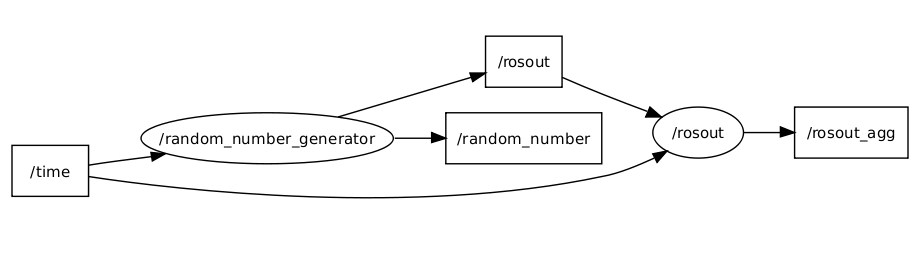
\includegraphics[width=.75\columnwidth]{rxgraph.png}
\begin{tabbing}
Us\=age:\\
\> \texttt{\$ rxgraph}\\
\end{tabbing}

\vspace{-1.5 mm}
\subsection{\href{http://www.ros.org/wiki/rxtools}{rxplot}}
A tool for plotting data from one or more ROS topic fields using matplotlib.\\
\vspace{2.5 mm}
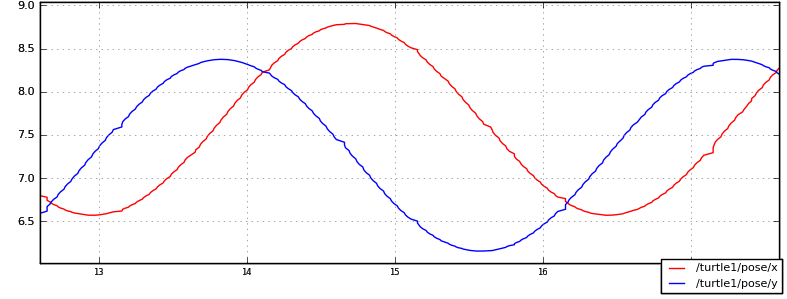
\includegraphics[width=.75\columnwidth]{rxplot.png}
\begin{tabbing}
E\=x\=amples:\\
\> To graph the data in different plots:\\
\> \>\texttt{\$ rxplot /topic1/field1 /topic2/field2}\\
\> To graph the data all on the same plot:\\
\> \>\texttt{\$ rxplot /topic1/field1,/topic2/field2}\\
\> To graph multiple fields of a message:\\
\> \>\texttt{\$ rxplot /topic1/field1:field2:field3}\\
\end{tabbing}

\vspace{-1.5 mm}
\subsection{\href{http://www.ros.org/wiki/rxbag}{rxbag}}
A tool for visualizing, inspecting, and replaying histories (bag files) of ROS messages.\\
\vspace{2.5 mm}
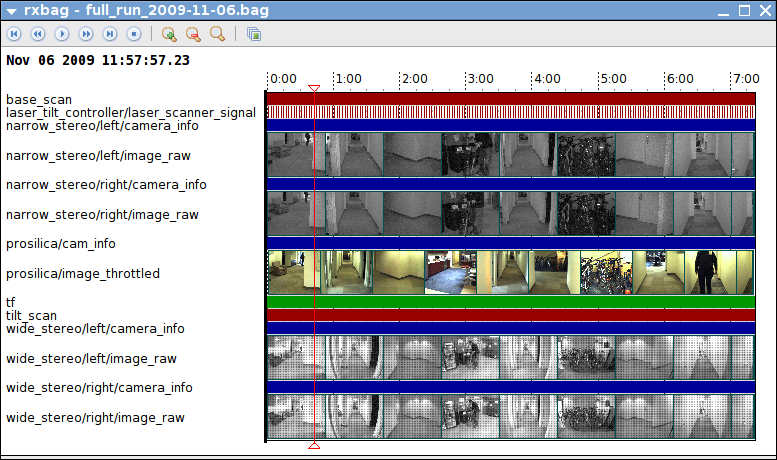
\includegraphics[width=.75\columnwidth]{rxbag-1.png}
\begin{tabbing}
Us\=age:\\
\> \texttt{\$ rxbag bag\_file.bag}\\
\end{tabbing}

\vspace{-1.5 mm}
\subsection{\href{http://www.ros.org/wiki/rxconsole}{rxconsole}}
A tool for displaying and filtering messages published on rosout.\\
\vspace{2.5 mm}
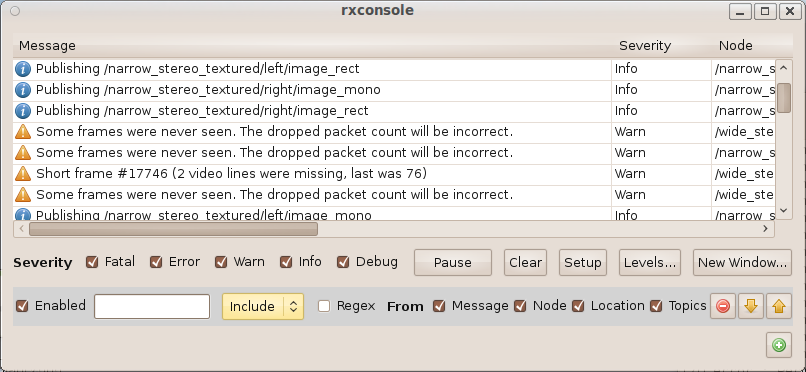
\includegraphics[width=.75\columnwidth]{rxconsole.png}
\begin{tabbing}
Us\=age:\\
\> \texttt{\$ rxconsole}\\
\end{tabbing}

\vspace{-2.5 mm}
\section{tf Command-line Tools}

\subsection{\href{http://www.ros.org/wiki/tf\#tf_echo}{tf\_echo}}
A tool that prints the information about a particular transformation between a source\_frame and a target\_frame.\\
\vspace{2.5 mm}
%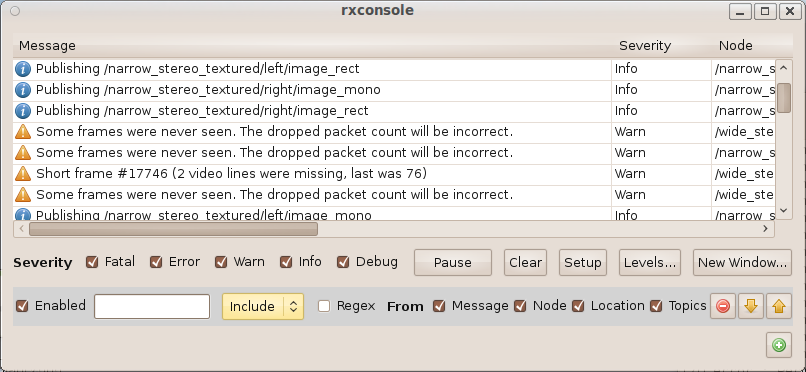
\includegraphics[width=.75\columnwidth]{rxconsole.png}
\begin{tabbing}
Us\=age:\\
\> \texttt{\$ rosrun tf tf\_echo <source\_frame> <target\_frame>}\\
\end{tabbing}
\begin{tabbing}
E\=x\=amples:\\
\> To echo the transform between /map and /odom:\\
\> \>\texttt{\$ rosrun tf tf\_echo /map /odom}\\
\end{tabbing}



\vspace{-1.5 mm}
\subsection{\href{http://www.ros.org/wiki/tf\#view_frames}{view\_frames}}
A tool for visualizing the full tree of coordinate transforms.\\
\vspace{2.5 mm}
%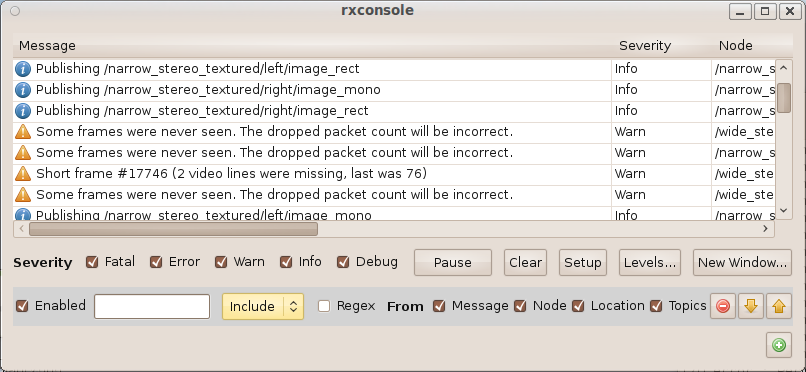
\includegraphics[width=.75\columnwidth]{rxconsole.png}
\begin{tabbing}
Us\=age:\\
\> \texttt{\$ rosrun tf view\_frames}\\
\> \texttt{\$ evince frames.pdf}
\end{tabbing}







\rule{0.3\linewidth}{0.25pt}
\scriptsize

Copyright \copyright\ 2013 Willow Garage
\vspace{3000 mm}


\end{multicols}
\end{document}
